

\documentclass[12pt,aspectratio=169]{beamer}

% Packages
\usepackage{mathtools}
\usepackage{hyperref}
\usepackage{setspace}
\usepackage{tikz}
\usetikzlibrary{positioning}
\usepackage{ragged2e}
\usepackage{nicematrix}
\usepackage[compatibility=false]{caption}
\usepackage[framemethod=tikz]{mdframed}

% Colored boxes
\usepackage{tcolorbox}
\tcbsetforeverylayer{autoparskip} % Removes unwanted vertical space

% Theme
\usetheme{metropolis}
\metroset{subsectionpage=progressbar,sectionpage=none}
\setbeamertemplate{theorems}[numbered]

\usepackage{fontspec}
\defaultfontfeatures{LetterSpace=30}


% Code
\usepackage{listings}
% Custom colors
\definecolor{codegreen}{rgb}{0,0.6,0}
\definecolor{codegray}{rgb}{0.5,0.5,0.5}
\definecolor{codepurple}{rgb}{0.58,0,0.82}
\definecolor{backcolour}{rgb}{0.95,0.95,0.92}
\definecolor{light-gray}{gray}{0.95}
% Python style for highlighting
\newcommand\pythonstyle{\lstset{
		backgroundcolor=\color{white},
		language=Python,
		basicstyle=\ttfamily\footnotesize,
		morekeywords={self},              % Add keywords here
		keywordstyle=\color{blue},
		stringstyle=\footnotesize\color{deepgreen},
		commentstyle=\color{codegreen},
		showstringspaces=false,
		frame=tb,
		numbers=left,
		numbersep=5pt,
		numberstyle=\tiny\color{gray},
		columns=fullflexible,
		numbersep=5pt,
		aboveskip=1em,
		showtabs=false,
		tabsize=2,
		gobble=3
	}}

% Python environment
\lstnewenvironment{python}[1][]
{
	\pythonstyle
	\lstset{#1}
}
{}
% Python for inline
\newcommand\pythoninline[1]{{\pythonstyle\lstinline!#1!}}

% Tables and justification
\newcommand{\ra}[1]{\renewcommand{\arraystretch}{#1}}
\justifying

% Subfigures
\setbeamertemplate{caption}[numbered]
\usepackage[caption=false,font=footnotesize]{subfig}

% Colors
\setbeamercolor{uppercolgreen}{fg=white,bg=green!35}
\setbeamercolor{lowercolgreen}{fg=black,bg=green!10}
\setbeamercolor{uppercolred}{fg=white,bg=red!35}
\setbeamercolor{lowercolred}{fg=black,bg=red!10}
\setbeamercolor{uppercolblue}{fg=white,bg=blue!35}
\setbeamercolor{lowercolblue}{fg=black,bg=blue!10}
\definecolor{darkred}{rgb}{0.55, 0.0, 0.0}
\definecolor{darkpastelblue}{rgb}{0.47, 0.62, 0.8}
\definecolor{darkcerulean}{rgb}{0.03, 0.27, 0.49}
\definecolor{darkgreen}{rgb}{0.0, 0.55, 0.0}
\definecolor{deepblue}{rgb}{0,0,0.5}
\definecolor{deepred}{rgb}{0.6,0,0}
\definecolor{deepgreen}{rgb}{0,0.5,0}

% Matrix size
\usepackage{stackengine}
\stackMath
\def\sss{\scriptstyle \color{gray}}
\setstackgap{L}{12pt}
\def\stacktype{L}

% Mathematical commands
\newcommand{\vc}[1]{\boldsymbol{\mathbf{#1}}}
\newcommand{\pr}[1]{{#1\,}'}
\newcommand{\idx}[2]{{\color{darkpastelblue}[}#1{\color{darkpastelblue}]_{#2}}}
\newcommand{\shape}[2]{\stackunder{#1}{\sss #2}}
\DeclareMathOperator*{\argmax}{arg\,max}
\DeclareMathOperator*{\argmin}{arg\,min}

% Style commands
\newcommand{\myalert}[1]{{\color{darkred}\textbf{#1}}}

% White frame (for images)
\newenvironment{whiteframe}[1]{
	\setbeamercolor{background canvas}{bg=white}
	\begin{frame}{#1}
		}{
	\end{frame}
}

\setbeamerfont{frametitle}{size=\normalsize}
\setbeamertemplate{frametitle}[default][right]
{
}
%\setbeamercolor{frametitle}{fg=white,bg=black!75}

% No headline frame
\makeatletter
\newenvironment{noheadline}{
	\setbeamertemplate{headline}{}
	\addtobeamertemplate{frametitle}{\vspace*{-3.5\baselineskip}}{}
}{}
\makeatother

% Lists
\setbeamertemplate{itemize items}[triangle]

% Footnotes
\setbeamertemplate{footnote}%
{%
	\parindent 1.5em\noindent%
	\justifying\setstretch{0.7}%
	\hbox to 1em{\hfil\insertfootnotemark}\begin{scriptsize}\insertfootnotetext\end{scriptsize}\par%
}

% Footnote without number
\newcommand\blfootnote[1]{%
	\begingroup
	\renewcommand\thefootnote{}\footnote[frame]{\noindent#1}%
	\addtocounter{footnote}{-1}%
	\endgroup
}

% Theorems
\newcommand*{\theorembreak}{\usebeamertemplate{theorem end}\framebreak\usebeamertemplate{theorem begin}}
\newcounter{theo}[section]\setcounter{theo}{0}
\renewcommand{\thetheo}{\arabic{section}.\arabic{theo}}

\newenvironment{theo}[2][]{%
	\refstepcounter{theo}%
	\ifstrempty{#1}%
	{\mdfsetup{%
			frametitle={%
					\tikz[baseline=(current bounding box.east),outer sep=0pt]
					\node[anchor=east,rectangle,fill=red!10]
					{\strut Theorem~\thetheo};}}
	}%
	{\mdfsetup{%
			frametitle={%
					\tikz[baseline=(current bounding box.east),outer sep=0pt]
					\node[anchor=east,rectangle,fill=red!10]
					{\strut Theorem~\thetheo:~#1};}}%
	}%
	\mdfsetup{innertopmargin=5pt,linecolor=red!10,%
		linewidth=2pt,topline=true,%
		frametitleaboveskip=\dimexpr-\ht\strutbox\relax
	}
	\begin{mdframed}[]\relax%
		\label{#2}}{\end{mdframed}}

% The 2024 source used annotate-equations for optional visual labels.
% Keep the deck portable when that package is unavailable.
\newcommand{\eqnmarkbox}[3][]{#3}
\newcommand{\annotate}[4][]{}
\usepackage{subfig}

% Colors
\definecolor{titlecolor}{RGB}{245, 242, 238} 
\definecolor{drawgray}{HTML}{666666}
\definecolor{drawgray_l}{HTML}{F5F5F5}
\definecolor{drawblue}{HTML}{6C8EBF}
\definecolor{drawblue_l}{HTML}{DAE8FC}
\definecolor{drawgreen}{HTML}{82B366}
\definecolor{drawgreen_l}{HTML}{D5E8D4}
\definecolor{draworange}{HTML}{D79B00}
\definecolor{draworange_l}{HTML}{FFE6CC}
\definecolor{drawyellow}{HTML}{D6B656}
\definecolor{drawyellow_l}{HTML}{FFF2CC}
\definecolor{drawred}{HTML}{B85450}
\definecolor{drawred_l}{HTML}{EA6B66}
\definecolor{drawviolet}{HTML}{9673A6}
\definecolor{drawviolet_l}{HTML}{E1D5E7}

\tcbset{
	nndsblue/.style={colback=drawblue_l!35!white,colframe=drawblue,boxrule=0.8pt,arc=1mm},
	nndsgreen/.style={colback=drawgreen_l!35!white,colframe=drawgreen,boxrule=0.8pt,arc=1mm},
	nndsorange/.style={colback=draworange_l!35!white,colframe=draworange,boxrule=0.8pt,arc=1mm},
	nndsred/.style={colback=drawred_l!12!white,colframe=drawred,boxrule=0.8pt,arc=1mm}
}


\begin{document}

	{\usebackgroundtemplate{\tikz\node[opacity=0.4,inner sep=0]{
\includegraphics[width=\paperwidth,height=\paperheight]{images/header}};}%
	\begin{frame}[plain]
		\vspace{0.5cm}
		\title{\large \begin{spacing}{1.0}Neural Networks for Data Science\end{spacing}\vspace{0.25em}
			\normalsize \begin{spacing}{1.0}\textbf{Master's Degree in Data Science}\end{spacing}\vspace{0.5em}}
		\subtitle{\Large \textbf{Lecture 3: Linear regression and classification}}
		\date{
			{
\includegraphics[scale=0.8]{images/Uniroma1}}
		}
		\author{
			\setlength{\tabcolsep}{2pt}
			\begin{tabular}{rl}
				\textbf{Lecturer}: & S. Scardapane \\
			\end{tabular}
		}\titlepage
	\end{frame}
	}

\part{1}

\section{Introduction}

\section{Supervised learning}
\subsection{Setup and data splits}

\begin{frame}{Supervised learning}

	\begin{columns}[T,onlytextwidth]
		\begin{column}{0.49\textwidth}
			\begin{tcolorbox}[nndsblue,height=0.42\textheight]
				\textbf{\color{darkcerulean}Dataset}

				A set of $N$ input--target pairs:
				\begin{equation}
					\mathcal{S}=\left\{(x_i,y_i)\right\}_{i=1}^{N} \,.
				\end{equation}
			\end{tcolorbox}
		\end{column}
		\begin{column}{0.49\textwidth}
			\begin{tcolorbox}[nndsgreen,height=0.42\textheight]
				\textbf{\color{darkgreen}Model}

				A map from an input to a prediction:
				\begin{equation}
					\hat{y}=f_{\boldsymbol{\theta}}(x) \,.
				\end{equation}
			\end{tcolorbox}
		\end{column}
	\end{columns}

	\vspace{1em}
	We fit $\boldsymbol{\theta}$ on $\mathcal{S}$ and evaluate the model on examples that were not used for training.

\end{frame}

\begin{frame}{Training, validation, and test data}

	\small
	We split the available examples into three disjoint sets:
	\begin{equation}
		\mathcal{S}
		= {\color{darkred}\mathcal{S}_{\mathrm{train}}}
		\mathbin{\dot\cup} {\color{darkpastelblue}\mathcal{S}_{\mathrm{val}}}
		\mathbin{\dot\cup} {\color{darkgreen}\mathcal{S}_{\mathrm{test}}} \,.
	\end{equation}

	\begin{columns}[T,onlytextwidth]
		\begin{column}{0.32\textwidth}
			\begin{tcolorbox}[nndsred,height=0.27\textheight]
				\textbf{\color{darkred}Training}

				Fit parameters $\boldsymbol{\theta}$.
			\end{tcolorbox}
		\end{column}
		\begin{column}{0.32\textwidth}
			\begin{tcolorbox}[nndsblue,height=0.27\textheight]
				\textbf{\color{darkcerulean}Validation}

				Choose model and hyperparameters.
			\end{tcolorbox}
		\end{column}
		\begin{column}{0.32\textwidth}
			\begin{tcolorbox}[nndsgreen,height=0.27\textheight]
				\textbf{\color{darkgreen}Test}

				Final evaluation.
			\end{tcolorbox}
		\end{column}
	\end{columns}

	\begin{tcolorbox}[nndsorange,boxsep=1mm,top=1mm,bottom=1mm]
		We usually assume i.i.d. samples from the same unknown distribution $p(x,y)$. If the deployment distribution differs, we have a \myalert{distribution shift}.
	\end{tcolorbox}

\end{frame}

\subsection{Loss functions}

\begin{whiteframe}{What is a good approximation?}
	
	\begin{figure}
		\centering
		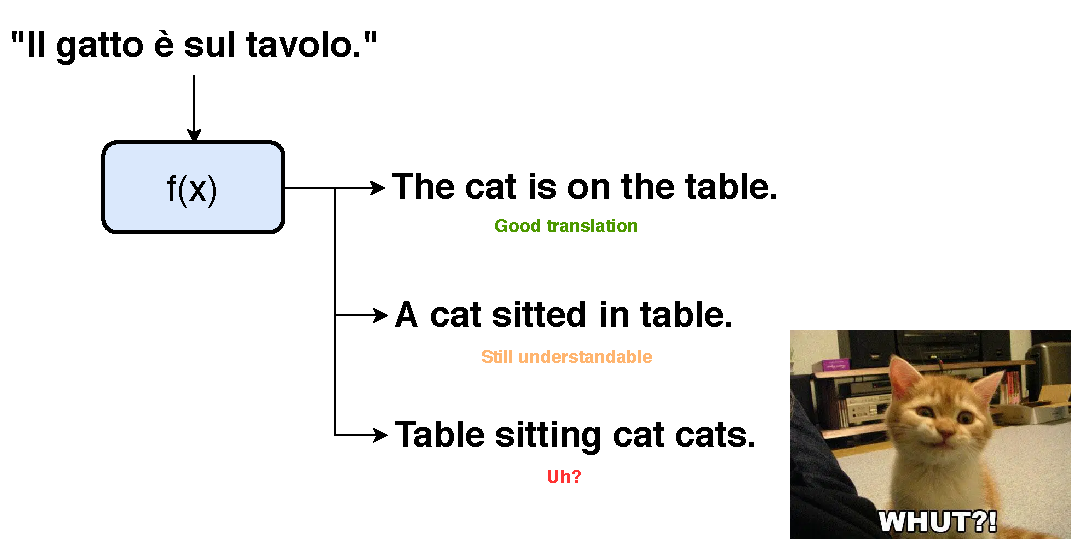
\includegraphics[width=1.0\columnwidth]{images/lecture_3/Lecture_2_different_translations}
	\end{figure}
	
\end{whiteframe}

\begin{frame}{Introducing loss functions}

	\begin{tcolorbox}[nndsblue]
		A \myalert{loss function} assigns a scalar cost to a prediction--target pair:
		\begin{equation}
			\ell\left(\hat{y}, y\right) \in \mathbb{R},
			\qquad \hat{y} = f_{\boldsymbol{\theta}}(x) \,.
		\end{equation}
	\end{tcolorbox}

	A smaller loss means a better prediction. Learning amounts to choosing $\boldsymbol{\theta}$ so that predictions have low loss on the training data.

	\begin{tcolorbox}[nndsgreen,boxsep=1mm,top=1mm,bottom=1mm]
		For gradient-based learning, we usually choose losses that are \myalert{differentiable} with respect to the model parameters.
	\end{tcolorbox}
	
\end{frame}

\begin{frame}{Expected risk and empirical risk}

	\small
	\begin{columns}[T,onlytextwidth]
		\begin{column}{0.49\textwidth}
			\begin{tcolorbox}[nndsgreen,height=0.61\textheight]
				\textbf{\color{darkgreen}What we care about}

				The loss over the full data distribution:
				\begin{equation}
					\mathcal{R}(\boldsymbol{\theta})
					=\mathbb{E}_{p(x,y)}\!\left[
					\ell\left(f_{\boldsymbol{\theta}}(x),y\right)\right] \,.
				\end{equation}
				This is the \myalert{expected risk}, but $p(x,y)$ is unknown.
			\end{tcolorbox}
		\end{column}
		\begin{column}{0.49\textwidth}
			\begin{tcolorbox}[nndsblue,height=0.61\textheight]
				\textbf{\color{darkcerulean}What we can optimize}

				The average loss over the training data:
				\begin{equation}
					\mathcal{L}(\boldsymbol{\theta})
					=\frac{1}{N}\sum_{i=1}^{N}
					\ell\left(f_{\boldsymbol{\theta}}(x_i),y_i\right) \,.
				\end{equation}
				\begin{equation}
					\boldsymbol{\theta}^*
					=\argmin_{\boldsymbol{\theta}}\mathcal{L}(\boldsymbol{\theta}) \,.
				\end{equation}
			\end{tcolorbox}
		\end{column}
	\end{columns}

	\begin{tcolorbox}[nndsorange,boxsep=1mm,top=1mm,bottom=1mm]
		A small empirical risk does not guarantee a small expected risk. Their difference is the \myalert{generalization gap}.
	\end{tcolorbox}
	
\end{frame}

\begin{frame}{Overfitting}

	\small
	Consider a model that memorizes the training set:
	\begin{equation}
		f(x) =
		\begin{cases}
			{\color{darkred}y_i}
			& \text{if } x=x_i \text{ for some } (x_i,y_i)\in\mathcal{S}_{\mathrm{train}}, \\
			{\color{darkpastelblue}\bar{y}}
			& \text{otherwise}.
		\end{cases}
		\label{eq:lookup_table}
	\end{equation}

	It predicts every training target exactly. For any new input, however, it returns the same default value $\bar{y}$.

	\begin{tcolorbox}[nndsorange,boxsep=1mm,top=1mm,bottom=1mm]
		Zero training risk does not imply small expected risk:
		\begin{equation*}
			{\color{darkred}\mathcal{L}(\boldsymbol{\theta})=0}
			\quad\nRightarrow\quad
			{\color{darkpastelblue}\mathcal{R}(\boldsymbol{\theta})\text{ is small}} \,.
		\end{equation*}
	\end{tcolorbox}

	This is \myalert{overfitting}: fitting the training data without learning a rule that generalizes.
	
\end{frame}

\begin{frame}{Losses for regression}

	\footnotesize
	For \myalert{regression} we have $y,\hat{y}\in\mathbb{R}$, and we can write the prediction error as $e=\hat{y}-y$.

	\begin{columns}[T,onlytextwidth]
		\begin{column}{0.43\textwidth}
			\begin{itemize}
				\item \textcolor{drawred}{\textbf{Squared loss}}:
				${\color{drawred}\ell(e)=e^2}$. Smooth, but gives large errors more weight.

				\item \textcolor{drawgreen}{\textbf{Absolute loss}}:
				${\color{drawgreen}\ell(e)=\lvert e\rvert}$. Less sensitive to outliers, but not differentiable at $e=0$.

				\item \textcolor{drawblue}{\textbf{Huber loss}}:
				quadratic near zero and linear for large $\lvert e\rvert$.
			\end{itemize}
		\end{column}
		\begin{column}{0.54\textwidth}
			\centering
			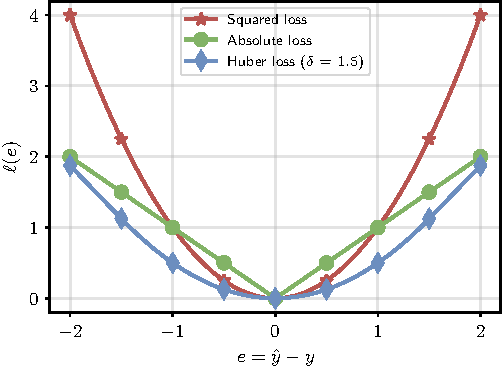
\includegraphics[width=0.94\linewidth]{images/lecture_3/loss_functions_regression.pdf}
		\end{column}
	\end{columns}

	\vspace{0.15em}
	{\scriptsize Maximum likelihood gives squared loss under Gaussian noise and absolute loss under Laplace noise, see the book.}

\end{frame}

\section{Linear models}
\subsection{Linear models for regression}

\begin{frame}{A linear model}

	\begin{tcolorbox}[nndsblue,boxsep=1mm,top=1mm,bottom=1mm]
		\justifying
		For an input $\vc{x}\in\mathbb{R}^{D}$, a scalar linear model is defined as:
		\begin{equation}
			f_{\boldsymbol{\theta}}(\vc{x})
			= {\color{darkpastelblue}\vc{w}^{\top}\vc{x}}
			  {\color{darkred}+\,b}
			= \sum_{j=1}^{D}w_jx_j+b \,.
		\end{equation}
		The parameters are $\vc{w}\in\mathbb{R}^{D}$ and $b\in\mathbb{R}$, with $\boldsymbol{\theta}=\{\vc{w},b\}$. The scalar $b$ is the \myalert{bias}; we will sometimes omit it to simplify the notation. We call each component $x_j$ a \myalert{feature}, and datasets of this form \myalert{tabular}.
	\end{tcolorbox}

\end{frame}

\begin{frame}{Least squares}

	\justifying
	With the bias omitted, we collect all $N$ training examples as rows of a matrix $\vc{X}$ and the  targets as a vector $\vc{y}$:
	\begin{equation}
		\vc{X}\in\mathbb{R}^{N\times D},
		\qquad \vc{y}\in\mathbb{R}^{N},
		\qquad \idx{\vc{X}}{i}=\vc{x}_i^{\top} \,.
	\end{equation}

	\begin{tcolorbox}[nndsblue]
		Combining a linear model with squared loss gives the \myalert{least-squares} objective:
		\begin{equation}
			\mathcal{L}_{\mathrm{LS}}(\vc{w})
			= \frac{1}{N}\sum_{i=1}^{N}
			\left(y_i-\vc{w}^{\top}\vc{x}_i\right)^2
			= \frac{1}{N}\left\lVert\vc{y}-\vc{X}\vc{w}\right\rVert^2 \,.
		\end{equation}
	\end{tcolorbox}

	For gradient descent we have $\nabla \mathcal{L}_{\mathrm{LS}}(\vc{w}) = \frac{2}{N}\vc{X}^{\top}(\vc{X}\vc{w}-\vc{y})$.

\end{frame}

\begin{frame}{Solving least squares}

	\small
	\begin{tcolorbox}[nndsblue]
		\textbf{\color{darkcerulean}Normal equations}

		For least squares, setting $\nabla \mathcal{L}_{\mathrm{LS}}(\vc{w})=\mathbf{0}$ gives a linear system:
		\begin{equation}
			\vc{X}^{\top}\vc{X}\vc{w}=\vc{X}^{\top}\vc{y} \,.
		\end{equation}
	\end{tcolorbox}

	\begin{tcolorbox}[nndsgreen]
		\textbf{\color{darkgreen}If $\vc{X}$ has full column rank}
		\begin{equation}
			\vc{w}^{*}=\left(\vc{X}^{\top}\vc{X}\right)^{-1}
			\vc{X}^{\top}\vc{y} \,.
		\end{equation}
	\end{tcolorbox}

	\begin{tcolorbox}[nndsorange,boxsep=1mm,top=1mm,bottom=1mm]
		Solving the $D\times D$ system directly costs roughly $\mathcal{O}(D^3)$. Gradient methods avoid the explicit solution, scale to larger problems, and still work when no closed-form solution is available.
	\end{tcolorbox}


\end{frame}

\begin{frame}{Regularizing least squares}

	\justifying
	\small
	With strongly correlated features, the fitted weights can be unstable.

	\begin{tcolorbox}[nndsorange,boxsep=1mm,top=1mm,bottom=1mm]
		\justifying
		\myalert{Regularization} modifies the training objective to favour solutions with useful properties. \myalert{Ridge regression} favours smaller weights:
		\begin{equation}
			\mathcal{L}_{\mathrm{ridge}}(\vc{w})
			= \frac{1}{N}\left(
			\left\lVert\vc{y}-\vc{X}\vc{w}\right\rVert^2
			{\color{darkred}+\,\lambda\left\lVert\vc{w}\right\rVert^2}
			\right) \,.
		\end{equation}
	\end{tcolorbox}

	At $\lambda=0$ this is ordinary least squares. Larger values produce smaller, more stable weights at the cost of training fit. Since the penalty acts on the coefficients, features should be on comparable scales.

	The normal equations and their solution become:
	\begin{equation}
		\left(\vc{X}^{\top}\vc{X}{\color{darkred}+\,\lambda\vc{I}}\right)\vc{w}^{*}
		= \vc{X}^{\top}\vc{y},
		\qquad
		\vc{w}^{*}
		= \left(\vc{X}^{\top}\vc{X}{\color{darkred}+\,\lambda\vc{I}}\right)^{-1}
		\vc{X}^{\top}\vc{y} \,.
	\end{equation}

\end{frame}

\subsection{Linear models for classification}

\begin{frame}{Linear models for classification}

	\justifying
	In classification, each target $y_i\in\{1,\ldots,C\}$ identifies one of $C$ classes. These numbers are labels, not quantities: class $2$ does not mean twice class $1$.

	A linear classifier produces one score for each class:
	\begin{tcolorbox}[nndsblue]
		\begin{equation}
			\vc{z}_i=\vc{W}\vc{x}_i+\vc{b}\in\mathbb{R}^{C},
			\qquad
			\vc{W}\in\mathbb{R}^{C\times D},
			\quad
			\vc{b}\in\mathbb{R}^{C} \,.
		\end{equation}
		The components of $\vc{z}_i$ are called the \myalert{logits}.
	\end{tcolorbox}

	\begin{tcolorbox}[nndsorange,boxsep=1mm,top=1mm,bottom=1mm]
		The largest logit gives the predicted class. Since $\argmax$ is not differentiable, training replaces the argmax with a continuous approximation (\myalert{softmax}) that turns the logits into probabilities.
	\end{tcolorbox}

\end{frame}

\begin{frame}{From logits to probabilities}

	\justifying
	\begin{tcolorbox}[nndsblue,boxsep=1mm,top=1mm,bottom=1mm]
		The \myalert{softmax} maps the logits to a vector $\vc{p}_i\in\mathbb{R}^{C}$:
		\begin{equation}
			\idx{\vc{p}_i}{k}
			=\idx{\operatorname{softmax}(\vc{z}_i)}{k}
			=\frac{\exp(z_{ik})}{\sum_{j=1}^{C}\exp(z_{ij})} \,.
		\end{equation}
	\end{tcolorbox}

	\begin{tcolorbox}[nndsgreen,boxsep=1mm,top=1mm,bottom=1mm]
		Every component is non-negative and the components sum to one:
		\begin{equation}
			\vc{p}_i\in\Delta_C
			=\left\{\vc{p}\in\mathbb{R}^{C}:p_k\geq 0,\ \sum_{k=1}^{C}p_k=1\right\} \,.
		\end{equation}
	\end{tcolorbox}

	We can therefore read $p_{ik}$ as the predicted probability of class $k$. Softmax preserves the ordering of the logits, so $\argmax_k p_{ik}=\argmax_k z_{ik}$.

\end{frame}

\begin{whiteframe}{Softmax and temperature}

	The \myalert{temperature} $\tau>0$ controls the sharpness of the distribution:
	\begin{equation}
		\idx{\operatorname{softmax}(\vc{z}/\tau)}{k}
		=\frac{\exp(z_k/\tau)}{\sum_{j=1}^{C}\exp(z_j/\tau)} \,.
	\end{equation}
	Smaller values produce sharper distributions; larger values produce flatter ones.
	The same temperature controls the sharpness of token distributions in language models.

	\begin{figure}
		\subfloat[Logits]{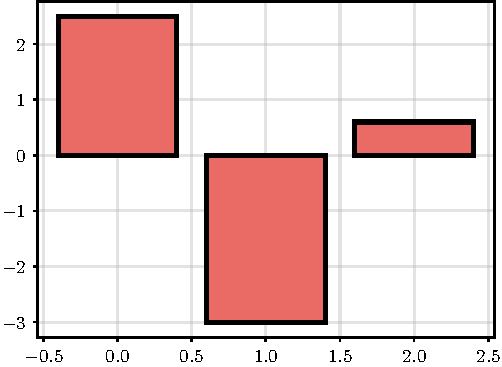
\includegraphics[width=0.19\columnwidth]{images/lecture_3/softmax_1.pdf}}\qquad
		\subfloat[$\tau=1$]{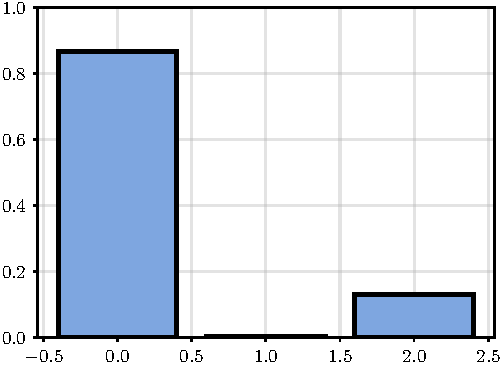
\includegraphics[width=0.19\columnwidth]{images/lecture_3/softmax_2.pdf}}\qquad
		\subfloat[$\tau=10$]{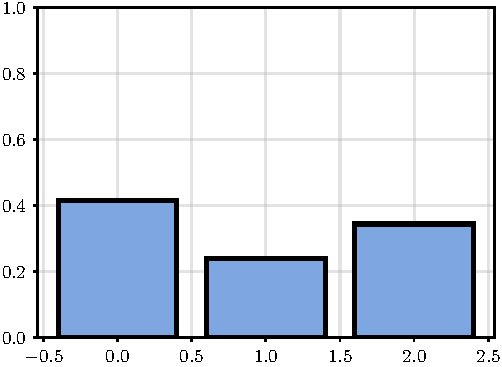
\includegraphics[width=0.19\columnwidth]{images/lecture_3/softmax_3.pdf}}\qquad
		\subfloat[$\tau=100$]{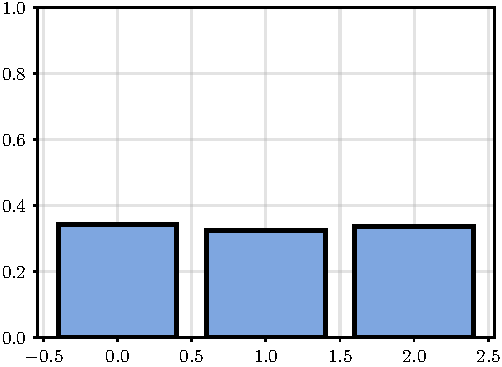
\includegraphics[width=0.19\columnwidth]{images/lecture_3/softmax_4.pdf}}
	\end{figure}

\end{whiteframe}

\begin{frame}{Multiclass logistic regression}

	\justifying
	\small
	Let $\vc{p}_i=f_{\boldsymbol{\theta}}(\vc{x}_i)$, with $\boldsymbol{\theta}=\{\vc{W},\vc{b}\}$.
	\begin{tcolorbox}[nndsblue]
		The \myalert{cross-entropy loss} is the negative log-probability assigned to the correct class:
		\begin{equation}
			\ell\left(f_{\boldsymbol{\theta}}(\vc{x}_i),y_i\right)
			=-\log p_{i,y_i} \,.
		\end{equation}
	\end{tcolorbox}

	With one-hot targets, this is the usual cross-entropy between two vectors.

	Training minimizes the empirical risk:
	\begin{equation}
		\mathcal{L}(\boldsymbol{\theta})
		=\frac{1}{N}\sum_{i=1}^{N}
		\ell\left(f_{\boldsymbol{\theta}}(\vc{x}_i),y_i\right) \,.
	\end{equation}
	There is no closed-form solution. The equivalent maximum-likelihood interpretation is discussed in the book.

\end{frame}

\begin{frame}{Binary classification}

	\justifying
	\begin{tcolorbox}[nndsblue,boxsep=1mm,top=1mm,bottom=1mm]
		For two classes, with $y_i\in\{0,1\}$, one scalar logit is enough:
		\begin{equation}
			s_i=\vc{w}^{\top}\vc{x}_i+b,
			\qquad
			p_i=\sigma(s_i)=\frac{1}{1+\exp(-s_i)} \,.
		\end{equation}
	\end{tcolorbox}
	Here $p_i$ is the probability of class $1$, while $1-p_i$ is the probability of class $0$.

	\begin{tcolorbox}[nndsgreen]
		The cross-entropy becomes the \myalert{binary cross-entropy}:
		%
		\begin{equation}
			\ell(p_i,y_i)
			=-y_i\log p_i-(1-y_i)\log(1-p_i) \,.
		\end{equation}
	\end{tcolorbox}

	The most probable class is $1$ whenever $p_i\geq 0.5$, equivalently whenever $s_i\geq 0$.

\end{frame}

\begin{frame}{What makes the classifier linear?}

	\footnotesize
	\begin{columns}[T,onlytextwidth]
		\begin{column}{0.49\textwidth}
			\begin{tcolorbox}[nndsblue,height=0.49\textheight]
				\textbf{\color{darkcerulean}Binary case}

				\justifying
				At threshold $0.5$, the predicted class changes when the scalar logit is zero:
				\begin{equation}
					\vc{w}^{\top}\vc{x}+b=0 \,.
				\end{equation}
				This hyperplane is normal to $\vc{w}$.
			\end{tcolorbox}
		\end{column}
		\begin{column}{0.49\textwidth}
			\begin{tcolorbox}[nndsblue,height=0.49\textheight]
				\textbf{\color{darkcerulean}Multiclass case}

				\justifying
				The boundary between classes $k$ and $j$ is where their logits are equal:
				\begin{equation}
					(\vc{w}_k-\vc{w}_j)^{\top}\vc{x}
					+(b_k-b_j)=0 \,.
				\end{equation}
				This is again a hyperplane.
			\end{tcolorbox}
		\end{column}
	\end{columns}

	\begin{tcolorbox}[nndsgreen,boxsep=1mm,top=1mm,bottom=1mm]
		\justifying
		Softmax and sigmoid are nonlinear, but the resulting decision boundaries are linear in the input. Curved boundaries require transforming or composing features, the topic of the next lecture.
	\end{tcolorbox}

\end{frame}

\begin{whiteframe}{Visualizing the sigmoid function}

	\begin{figure}
		\centering
		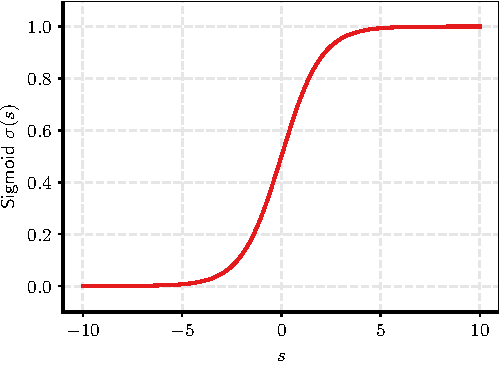
\includegraphics[width=0.6\columnwidth]{images/lecture_3/sigmoid.pdf}
		\vspace{-0.5em}\caption{The sigmoid approaches $0$ and $1$ asymptotically.}
	\end{figure}

\end{whiteframe}

\begin{frame}{Cross-entropy from logits}

	\justifying
	Computing softmax first and then taking its logarithm can be numerically unstable.
	\begin{tcolorbox}[nndsblue,boxsep=1mm,top=1mm,bottom=1mm]
		Substituting the softmax definition gives the equivalent logits-based loss:
		\begin{equation}
			\ell(\vc{z}_i,y_i)
			=-z_{i,y_i}+\operatorname{logsumexp}(\vc{z}_i) \,.
		\end{equation}
	\end{tcolorbox}

	\begin{tcolorbox}[nndsgreen,boxsep=1mm,top=1mm,bottom=1mm]
		Writing $m_i=\max_k z_{ik}$, we can evaluate the second term safely as:
		\begin{equation}
			\operatorname{logsumexp}(\vc{z}_i)
			=m_i+\log\sum_{k=1}^{C}\exp(z_{ik}-m_i) \,.
		\end{equation}
	\end{tcolorbox}

	Use logits-based framework losses; apply softmax only when probabilities are needed.

\end{frame}
\begin{frame}{Can we trust these probabilities?}

	\justifying
	Softmax scores are not automatically calibrated probabilities.

	\begin{tcolorbox}[nndsgreen,boxsep=1mm,top=1mm,bottom=1mm]
		\justifying
		A classifier is \myalert{calibrated} if predictions made with confidence $q$ are correct about a fraction $q$ of the time.
	\end{tcolorbox}

	\vspace{0.5em}
	\centering
	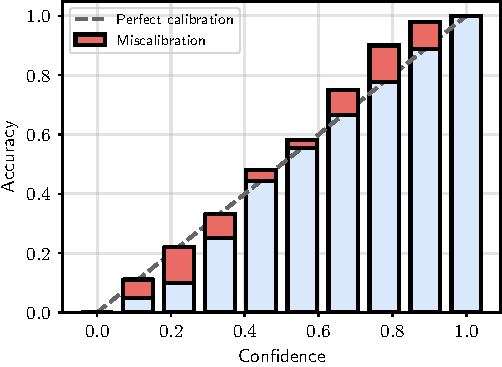
\includegraphics[width=0.38\columnwidth]{images/lecture_3/reliability_plot.pdf}
	\par\vspace{-0.2em}
	This is a \myalert{reliability plot}, see the book for more details.

\end{frame}
\begin{frame}{Reading material}
	
	\begin{itemize}
		\item \textbf{Chapters 3 and 4} of the book, along with the suggested exercises in Chapter 4.
	\end{itemize}
	
\end{frame}

\end{document}
